\section{Experimental Setup}

Figure~\ref{fig:evidence-pipeline} maps three distinct lanes before any claim is interpreted: Paper RQ1, the Fixed-cache demo, and the Live dual demo. Parallel model branches denote comparison alternatives rather than a model dependency. Protected-test access remains sealed throughout the pipeline.

Prospective RQ1-v2 index/integrity admission remains \texttt{blocked}. Its source-byte verification and rerun evidence are unavailable; it cannot replace historical Paper RQ1, fixed Loop206 cache evidence, or the reconstructed live display.

\begin{figure*}[t]
\centering
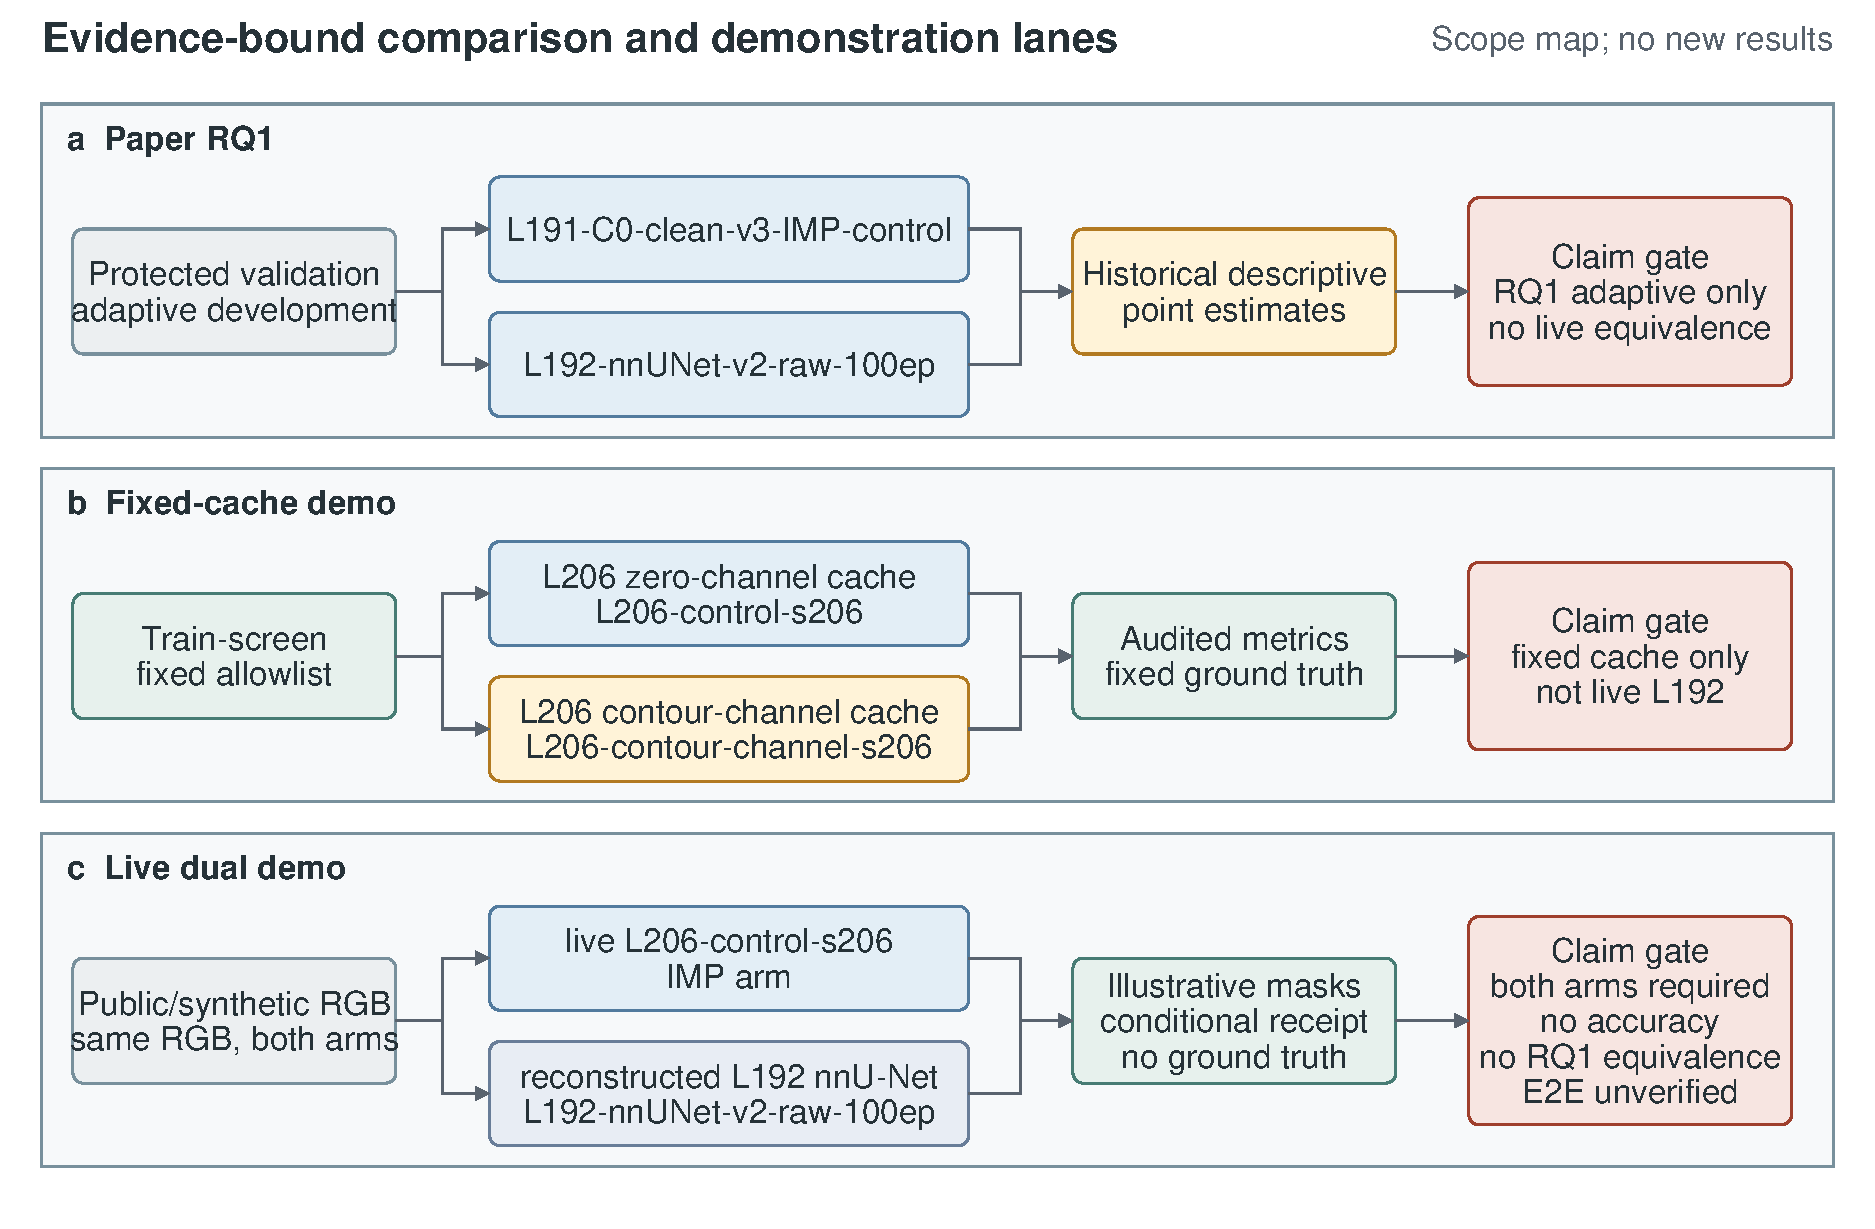
\includegraphics[width=\textwidth]{figures/evidence_pipeline.pdf}
\caption{Evidence-bound comparison and demonstration lanes. Paper RQ1, the fixed-cache demo, and the live dual demo use distinct inputs, model identities, outputs, and claim gates. Parallel arms are alternatives, not a sequential model chain. The figure supports protocol and claim-scope mapping only; it is not performance evidence.}
\label{fig:evidence-pipeline}
\end{figure*}

\subsection{Architecture comparison}

The historical Paper RQ1 comparison is L191-C0-clean-v3-IMP-control versus L192-nnUNet-v2-raw-100ep. Both use the same \cleanv{} validation identities and the six-condition robustness panel. That validation partition also informed iterative development, checkpoint or model selection, and promotion decisions, so the comparison is adaptive and potentially selection-optimistic rather than confirmatory. We report robust Dice, IoU, precision, recall, and boundary F1. Because each model has one recorded run and paired per-case evidence is not locally available in the rescue environment, no confidence interval or hypothesis test is attached to this table. Differences are descriptive point estimates.

Loop192 was evaluated against a preregistered combined promotion gate. Although its overlap and recall increased, it did not meet all boundary and precision constraints; the experiment stopped without test-v3 access. Gate failure is reported separately from metric ranking because an all-or-nothing promotion decision answers a different question from a Pareto comparison.

\subsection{Contour-channel ablation}

Loop206 uses three matched seeds. For each seed, the zero-channel control and contour-channel candidate are trained for 20 epochs on the fit portion of the 384-group train-only pilot and evaluated on the same 76 train-screen holdout groups under clean, low-contrast, and Gaussian-noise conditions. No protected image or mask participates in fitting, threshold calibration, checkpoint selection, or evaluation.

The primary endpoint is the paired candidate-minus-control robust Dice delta. Secondary endpoints include boundary F1, IoU, precision, recall, HD95, ASSD, empty predictions, and resource limits. For each split group, the procedure first averages paired candidate-minus-control deltas across the three selected seeds and three preregistered views. It then performs 10,000 paired bootstrap resamples of the 76 whole split groups. The interval preserves within-group view dependence but is conditional on the selected seeds; it does not estimate variability over seed selection.

The preregistered gate requires a positive primary effect with a positive lower confidence bound, Dice and boundary non-inferiority, clean Dice preservation, precision improvement, recall preservation, distance-metric safety, and bounded corruption regressions. Failure closes Loop206 without protected validation or test access.

\subsection{Compute}

Loop206 ran on an NVIDIA GeForce RTX 5060 Ti; preflight recorded 15.928 GiB total GPU memory. The final stage consumed 2,239.7 seconds, reached 15.644 GiB observed GPU use, 8.612 GiB process-group resident memory, and a 0.018 GiB maximum swap increase. These measurements describe the recorded run rather than a cross-platform efficiency benchmark.
